\subsection{Setup Requirements}

\begin{figure}[ht]
    \centering
    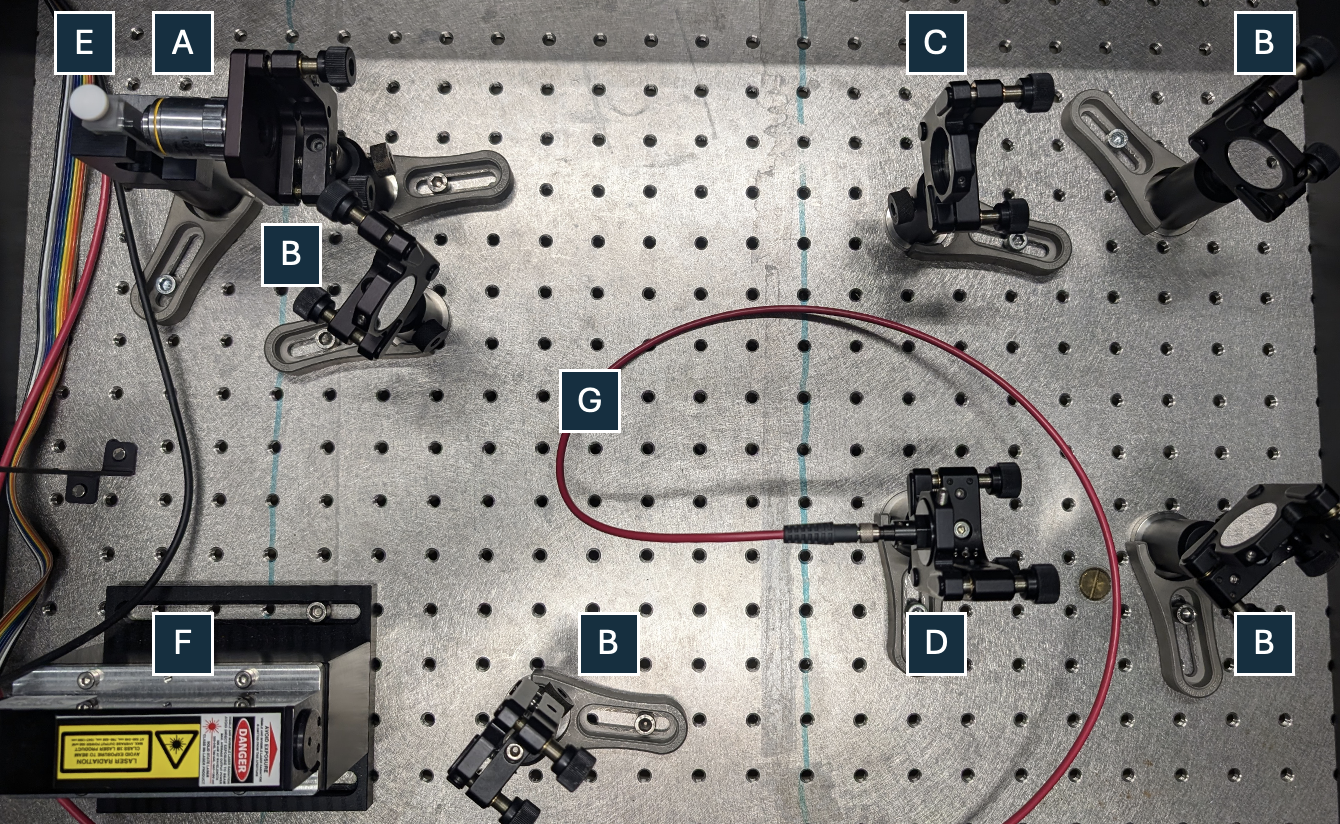
\includegraphics[width=\textwidth]{images/setup_graphics/setup_photo_numbered.png}
    \caption{Graphic of the setup used. A) Objective; B) Mirror; C) Notch filter; D) Optical fibre coupler; E) Sample; F) Laser; G) Optical Cable}
    \label{fig:setup_photo_numbered}
\end{figure}


\subsection{Setup}

\begin{figure}[ht]
    \centering
    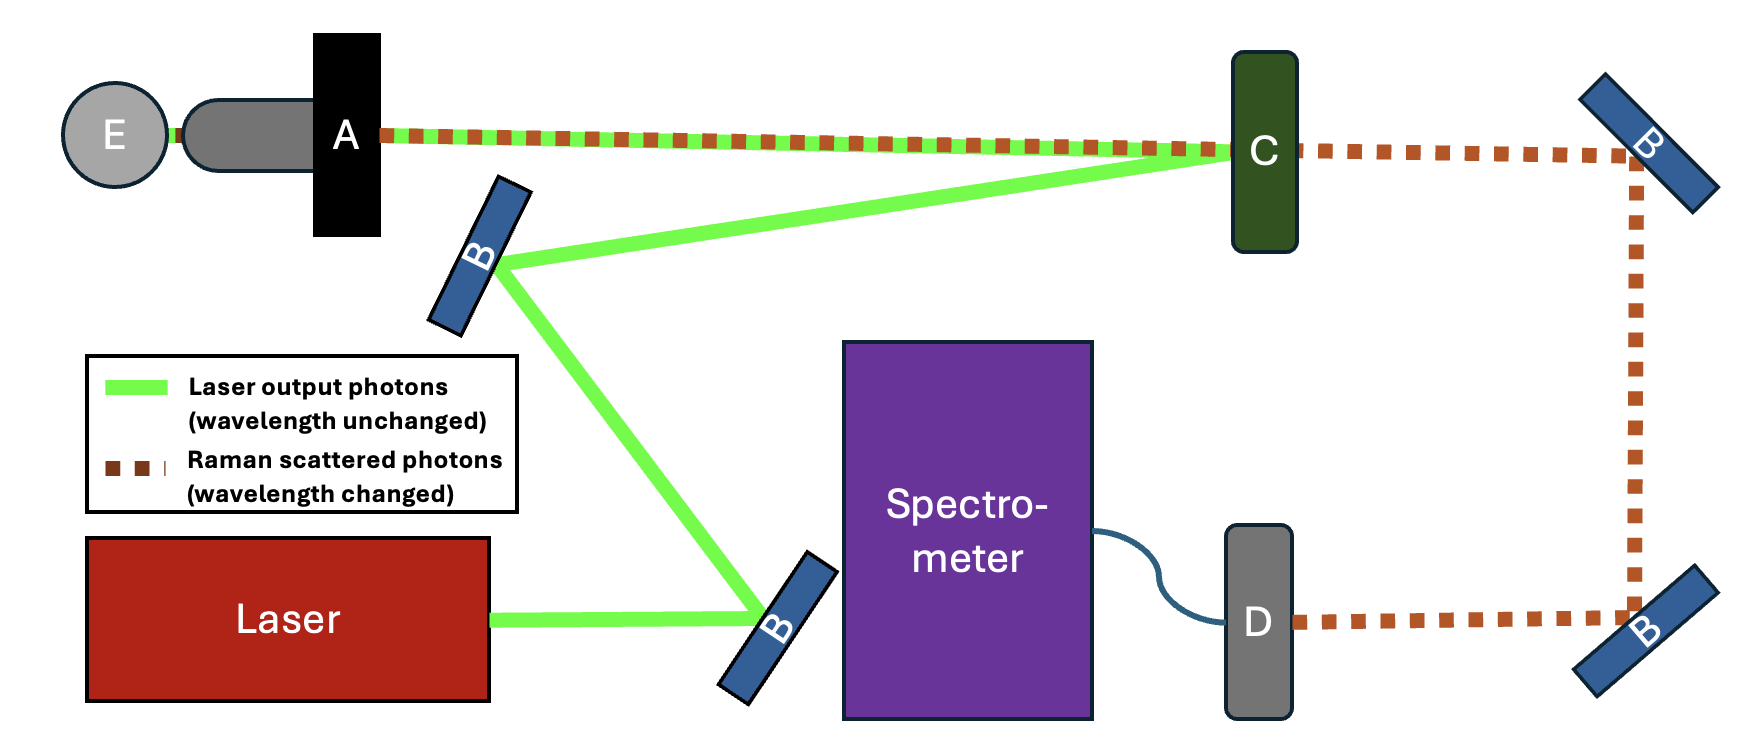
\includegraphics[width=\textwidth]{images/setup_graphics/setup_graphic.png}
    \caption{Graphic of a setup with the optical path. A) Objective; B) Mirror; C) Notch filter; D) Optical fibre coupler; E) Sample}
    \label{fig:setup_graphic}
\end{figure}

A setup for Raman spectroscopy (see Figure \ref{fig:setup_graphic}) uses a laser as the source of excitation radiation, since it has to be monochromatic in order for the raman scattered photons to be visible. By using several mirrors (B), the light is directed to a notch filter (C), which reflects almost all of the photons with a certain wavelength, which is notch-specific. The notch filter has to be selected so that it reflects the original (laser) wavelength. The reflected photons are directed towards a sample (E). Since only a small amount of photons get Raman scattered, it is essential to try to gather them efficiently, so an objective (A) is used to capture the photons, but also to focus the laser light onto the sample surface. The reflected and scattered light that passes back through the objective hits the notch filter again, where the Raman scattered photons pass through while the others get reflected. After passing through the notch filter, mirrors reflect the photons onto an optical fibre coupler, which collects them into an optic fibre to bring them to a spectrometer where they will get recorded as a spectrum.

\newpage

\subsubsection{Laser}
The acronym laser, which stands for "Light Amplification by Stimulated Emission of Radiation" was coined in 1959 by Gordon Gould.
A laser beam is a stream of photons, all of which have the same wavelength and phase. 

\bigskip

In quantum mechanics, electrons in atoms have certain discrete energy levels they can occupy. The higher the energy level, the more energy the atom has. Spontaneously, the atom can transition to a lower energy level, which is when the energy difference between the two levels is released in form of electromagnetic radiation, so a photon. This is called spontaneous emission. In contrast, stimulated emission when a passing photon interacts with the excited electron and causes it to transition to a lower energy level, which creates a photon. The passing photon has to have the same energy as the newly created one, and the created photon also has the same phase as the other. This creates a chain reaction, more and more photons are created if there are enough atoms in an excited state.\cite{wikilaser} \cite{wikistimlaser}

\bigskip

\begin{figure}[ht]
    \centering
    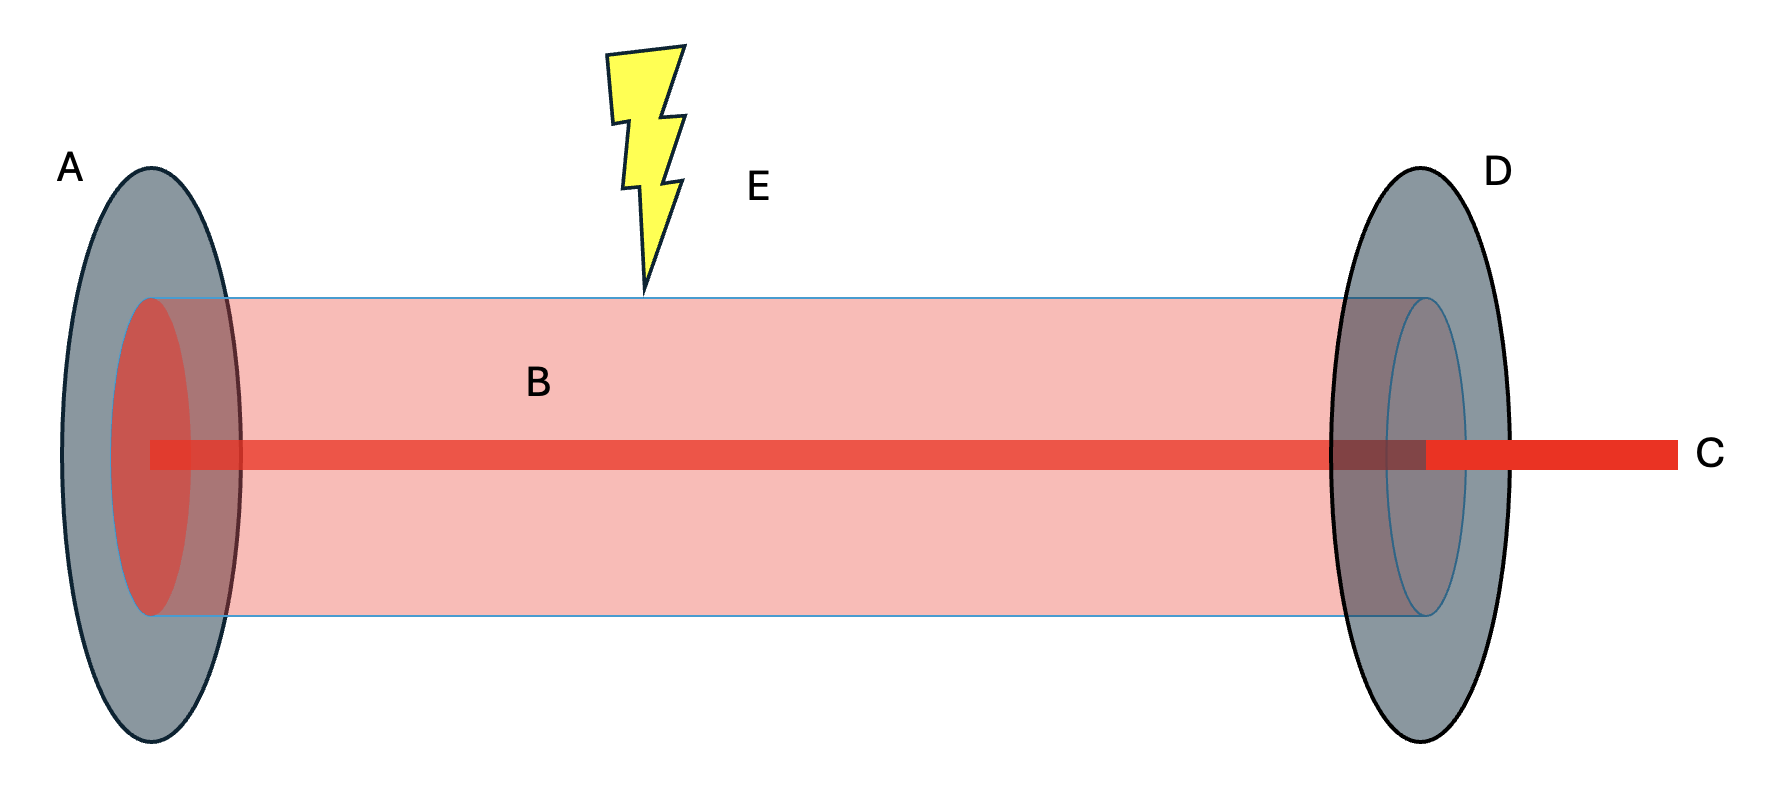
\includegraphics[width=\textwidth]{images/setup_graphics/laser.png}
    \caption{Graphic of a simplified laser: A) full mirror; B) gain medium; C) laser beam; D) partial mirror; E) laser pumping energy;}
    \label{fig:laser}
\end{figure}


In a typical laser (see Figure \ref{fig:laser}), energy (E) is pumped into a so called gain medium (B), usually either by an outside light source or electric field. This process is either continuous or pulsed. When the amount of atoms in one excited state exeeds that of atoms in some lower state, more photons are released than absorbed, the light is amplified. This state is called population inversion. The gain medium is placed between a full mirror (A), which reflects the photons, and a partial mirror (D), which lets some photons through. These photons make up the laser beam (C).\cite{wikilaser} \cite{wikistimlaser}

\newpage

\subsubsection{Notch Filter}
HELP

\newpage
\subsubsection{Optical Spectrometer}


\begin{figure}[ht]
    \centering
    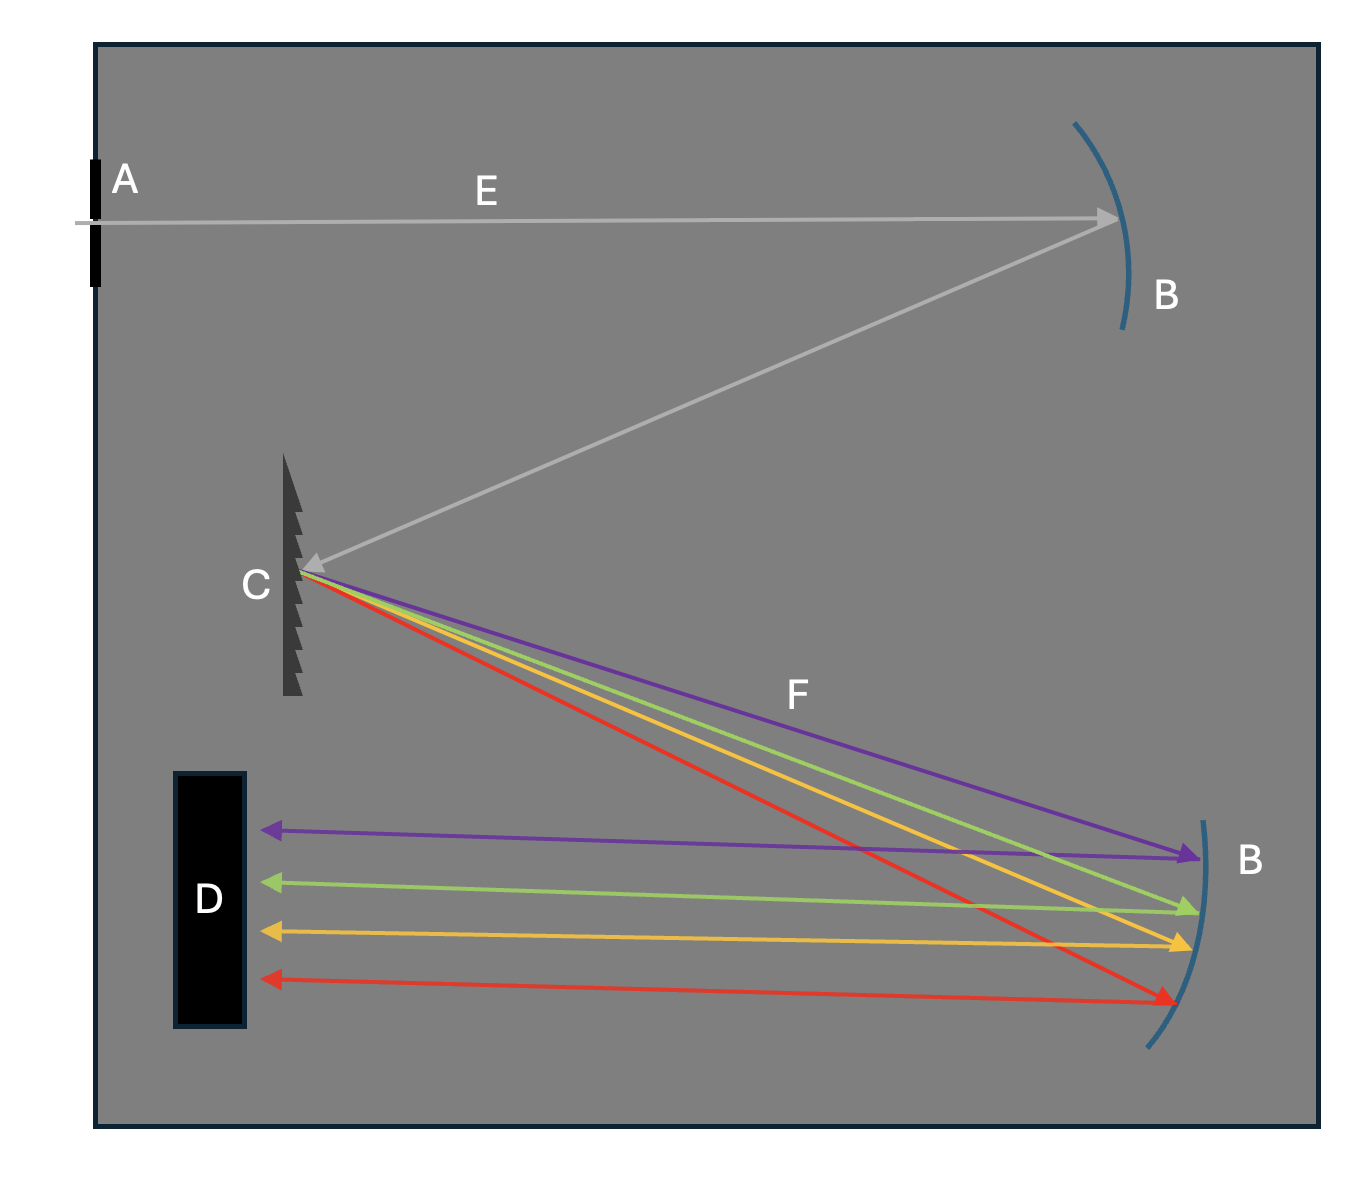
\includegraphics[width=0.9\textwidth]{images/setup_graphics/spectrometer.png}
    \caption{Graphic of a spectrometer A) Entrance slit; B) Mirrors; C) Optical grating; D) CCD detector; E) Incident light; F) Diffracted light}
    \label{fig:spectrometer}
\end{figure}

There exist different types of spectrometers, used to measure light intensity, charges, electron energies and other parameters of samples. Raman spectroscopy uses an opticl spectometer. An optical spectrometer is a device that is used to record and measure light intensity as a version its wavelength. This means that it separates light by wavelength over a fixed period of time. Some spectrometers can also measure the polarization of incident light, which can be used in certain types of Raman spectroscopy, it is specifically essential when Raman spectroscopy is used of crystals. \cite{RSAA} \cite{wikioptspec}

\bigskip

A typical spectrometer (see Figure \ref{fig:spectrometer}) functions in the following way: Light (E) enters the spectrometer through a small entrance slit (A). There it is reflected onto an optical grating (C), which will be discussed in the next chapter. This optical grating separates the light by wavelenghts (F), which are once again reflected onto a CCD detector (D). It records the incident photons and this paper will not address the way the CCD detector is built and the physics behind it's functions.\cite{wikigrating}

\paragraph{Optical Grating}

\begin{wrapfigure}{l}{0.4\textwidth} %this figure will be at the right
    \centering
    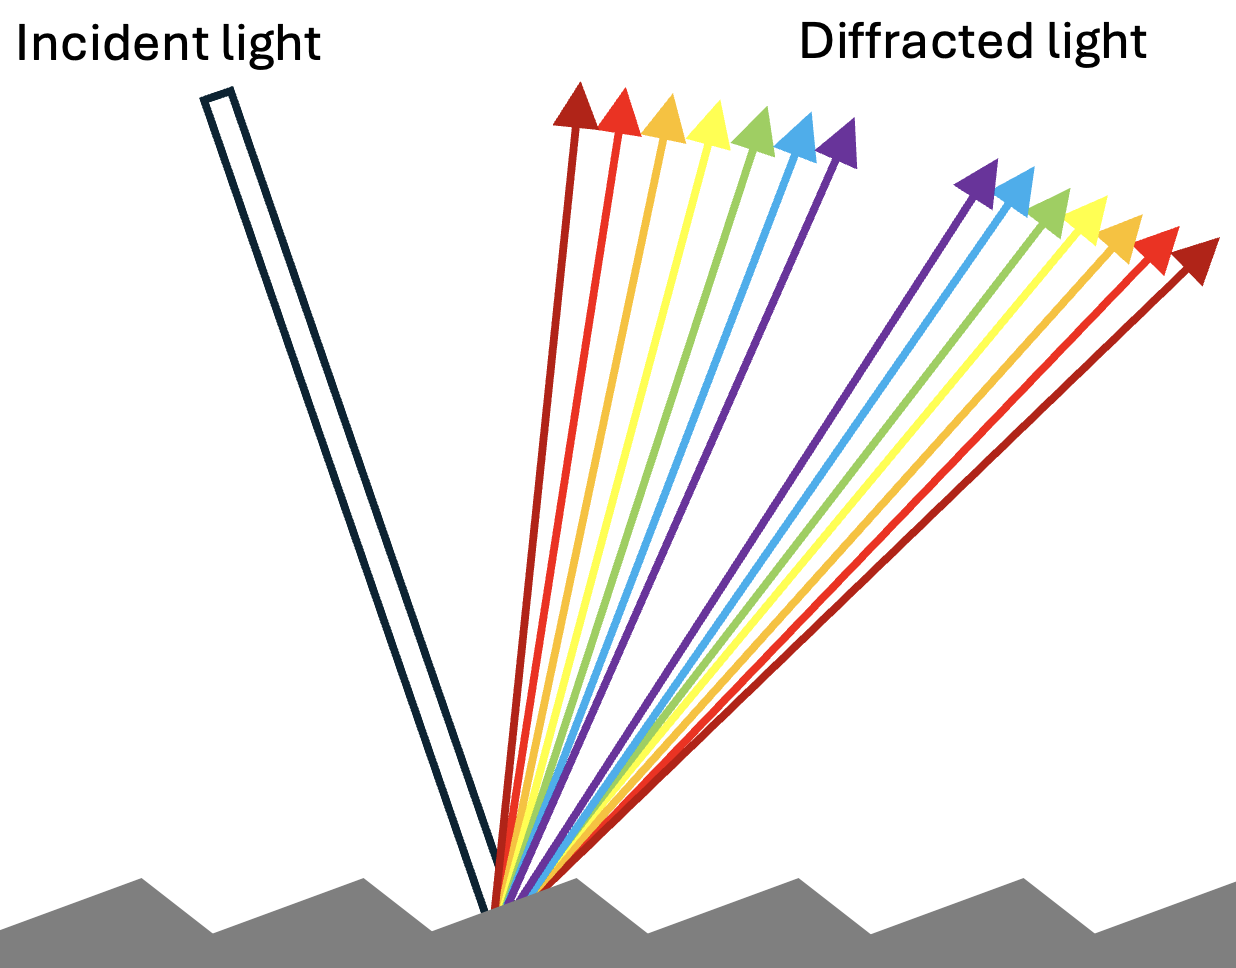
\includegraphics[width=0.3\textwidth]{images/setup_graphics/optical_grating.png}
    \caption{Graphic of an optical grating, simplified}
    \label{fig:grating}
    \vspace{-20pt}
\end{wrapfigure}

An optical grating is used to separate white light by wavelength. Generally, gratings can be separated into two types: reflection and transmission gratings. A reflection grating diffracts light back into the plane of incidence, while a transmission grating transmits it. 
\begin{wrapfigure}{r}{0.5\textwidth}
    \centering
    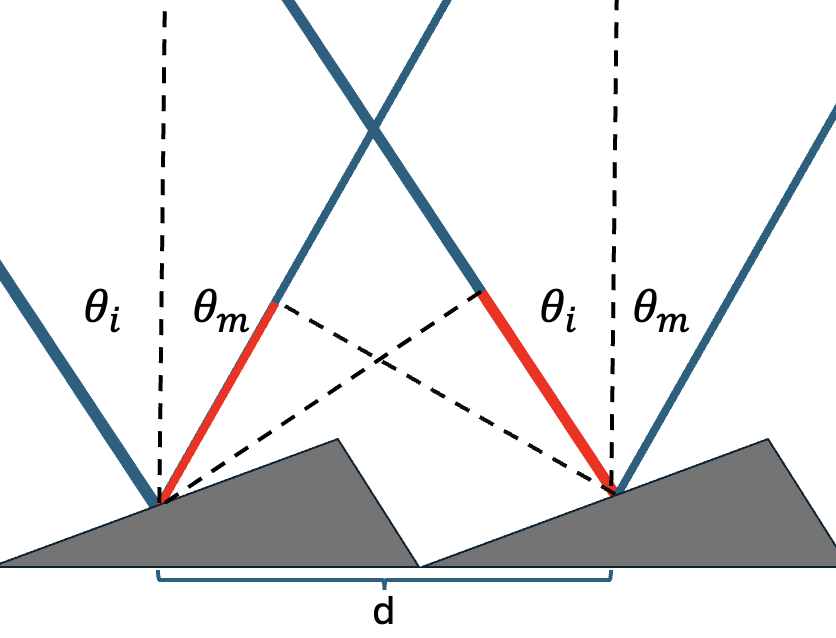
\includegraphics[width=0.4\textwidth]{images/setup_graphics/grating_graphic.png}
    \caption{Graphic of a reflection grating: d: distance between grooves, \(\theta_i\): incident angle light; \(\theta_m\): angle with constructive interference; Blue: distance in the path of both photons that is the same; Red: differences in path distance}
    \label{fig:grating_graphic}
\end{wrapfigure}
Figure \ref{fig:grating} depicts a reflection grating. Spectrometers usually use reflection gratings, they will be discussed.

\bigskip

A reflection based diffraction grating is a plate with grooves which are tightly spaced. The shape of the grooves can differ, Figure \ref{fig:grating} shows a triangular grooving, but mor wave-like groovings are also common. Generally, the distance between the grooves is not given but can be calculated from the usually given groove density value. Typical gratings have a groove density value between 30 and 5000 grooves per mm.

\bigskip


When photons hit a diffraction grating, they are diffracted into all directions. Since a photon is an electromagnetic wave with wavelength \(\lambda\), they interfere with each other. The interference can be constructive or destructive, depending on whether the waves are in phase or out of phase. In order to be constructive, the diffenrence in path of two photons of the same wavelength has to be a multiple of the wavelength. The angles at which the interference is constructive can be calculated with the wavelength, incident angle and groove spacing.


\begin{equation}
     sin(\theta_m)-sin(\theta_i)=\frac{m \lambda}{d}
 \end{equation}

\(\theta_i\): Incident angle (see Figure \ref{fig:grating_graphic})\\
\(\theta_m\): Diffraction angle (see Figure \ref{fig:grating_graphic})\\
m: Order of diffraction\\
\(\lambda\): Wavelength incident light\\
D: Distance beetween grooves (see Figure \ref{fig:grating_graphic})

\newpage

\subsection{Additional Material}

In addition, to properly align the mirrors, a second, much weaker laser was used. It was inserted in place of the optical fibre coupler and used to align the mirrors between the notch filter and the optical coupler. 

\bigskip

The intensity of the Raman shifted light which is reflected by those mirrors is too weak to be observed and used to align the mirrors, which is the reason the second laser was used. Its wavelength differs from the main laser so that it can pass through the notch filter which is chosen based on the wavelength of the main laser
\bigskip

While working with the laser, laser safety glasses were worn. 

\subsubsection{Laptop with OceanView 1.6.7}

\begin{wrapfigure}{r}{0.4\textwidth}
    \vspace{-20pt}
    \centering
    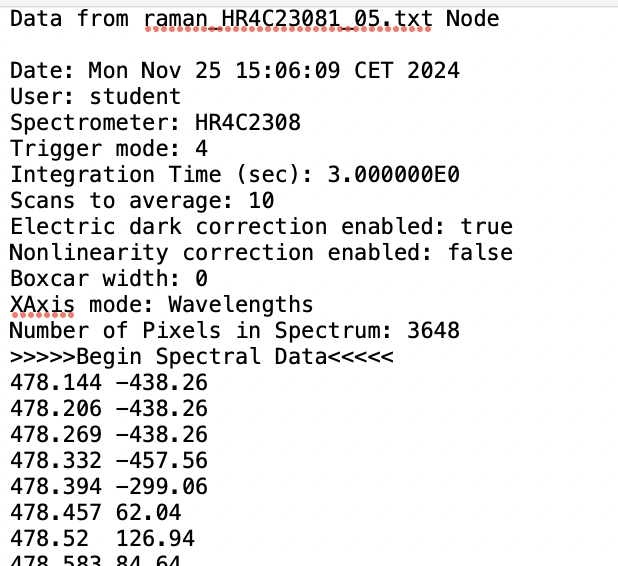
\includegraphics[width=0.4\textwidth]{images/data_raman.png}
    \vspace{-30pt}
    \caption{Beginning of the exported Raman data file}
    \label{fig:raman_txt}
    \vspace{-10pt}
\end{wrapfigure}
The spectrometer was connected to a laptop with the software OceanView 1.6.7, which was used to record spectra of the samples. The data points were exported as a text file, see Figure \ref{fig:raman_txt}. The file contains information to the data, when it was recorded, what integration time was used and how many scans were averaged out, among other parameters. The spectral data is then evaluated and plotted using python code, see Figure \ref{fig:python} in the Appendix.

\bigskip

